\documentclass[12pt,oneside]{article}
\usepackage{enumerate}
\usepackage{fancyhdr}
\usepackage{a4wide}
\usepackage{titlesec}
\usepackage{enumitem}
\usepackage[utf8]{inputenc}
\usepackage{graphicx} % Required for inserting images
\usepackage{tocloft}
\usepackage[table]{xcolor}
\usepackage{ragged2e}

\setlength{\arrayrulewidth}{0.5mm}
\setlength{\tabcolsep}{10pt}
\renewcommand{\arraystretch}{2.5}

\usepackage{longtable}
\definecolor{lightblue}{HTML}{b0c4de}
\definecolor{lightsteelblue}{HTML}{add8e6}

\usepackage{hyperref}

\usepackage{floatrow} 
\usepackage{graphicx}
\usepackage[export]{adjustbox}
\usepackage{wrapfig}
\usepackage{subcaption}

%%%%%%%%%%%%%%%%%%%%%%%%%%%%%%%%
\begin{document}

%pagina introduttiva
\begin{titlepage}
    \begin{flushright}
        \textbf{Corso di Fondamenti di Intelligenza Artificiale}
        \textbf{\\Università degli Studi di Salerno}
    \end{flushright}
    \vspace*{1.5cm}
    \centering
    \includegraphics[width=0.4\textwidth]{pics/logoUNISA.png}
    \vfill
    \Huge\textbf{BOOKS}
    \vspace{1ex}
    \rule{\linewidth}{1pt}
    \Large\textbf{Maria Angela Mancuso \\
        Ines Malfettone \\
        Federico Santonicola \\
        Attilio Sessa}
    \vfill
    \today
\end{titlepage}

%indice
\clearpage %crea nuova pagina

\setcounter{page}{1}

\begin{flushright}
        \Large\textbf{Indice}
\end{flushright}
\rule{\linewidth}{1pt}

\renewcommand{\contentsname}{}
\tableofcontents

%1
\clearpage
\setcounter{section}{0}
\section{Introduzione}
    \begin{enumerate}
    \subsection{Scopo del progetto}
    \begin{justify}

        Il nostro progetto si pone come obiettivo lo studio e la sperimentazione di differenti tecniche di Machine Learning capaci di analizzare ed estrarre informazioni da dati sotto forma di linguaggio naturale. Nello specifico si è interessati alla categorizzazione di libri tramite una breve descrizione testuale ed un elenco di autori. La categorizzazione è stata elaborata tramite due tecniche di Machine Learning, Classificazione e Clustering, che, seppur facenti utilizzo di due approcci diversi (rispettivamente apprendimento supervisionato e apprendimento non supervisionato), in linea teorica dovrebbero essere in grado di riportare risultati similari e confrontabili. A tal proposito occorrerà addestrare più modelli differenti per entrambe le tecniche e verificare quali di questi permette di ottenere il miglior risultato.

    \end{justify}
    \end{enumerate}

\hfill
\hfill
\section{Specifiche del progetto}
    \begin{enumerate}
        \subsection{Ambiente: PEAS}
   
%tabella
    \centering
    \begin{longtable}{ | p{3cm} | p{11cm} | }\hline
    \multicolumn{2}{|c|}{PEAS} \\ \hline
    \rowcolor{lightblue}
    Performance & La misura di prestazione è la capacità di avvicinarsi quanto più possibile al corretto genere del libro in questione. È necessario utilizzare misure di prestazione differenti per valutare Classificazione e Clustering. Nel caso della Classificazione si è usato: Accuratezza, Report di classificazione, che comprendono Precisione, Recall e F1-score per ciascuna classe, e una Matrice di  confusione. Per il clustering, invece,  si è utilizzato il Silhouette Score.\\
    \hline
    \rowcolor{lightsteelblue}
    \textbf{Environment} & I nostri modelli sono stati realizzati e operano nell'ambiente di sviluppo PyCharm il quale presenta le seguenti caratteristiche: \begin{itemize}
        \item \textbf{completamente osservabile}: il modello ha la visione completa del dataset e degli attributi associati a ciascun libro.
        \item \textbf{deterministico}: una volta addestrato un modello, la variazione dello stato dell'ambiente rimane la stessa a fronte degli stessi input.
        \item \textbf{episodico}: l'agente delibera a fronte di determinati episodi che consistono in nuove richieste di predizione.
        \item \textbf{statico}: l'ambiente resta invariato mentre l'agente opera.
        \item \textbf{discreto}: viene fornito un insieme discreto di informazioni per ciascun libro.
        \item \textbf{singolo}: l'ambiente permette di addestrare più modelli ma questi vengono valutati singolarmente.
    \end{itemize}
    \hline
    \rowcolor{lightblue}
    \textbf{Actuators} & Gli agenti mostrano i risultati attraverso due tipi di attuatori: \begin{itemize}
    \item console dell'ambiente di sviluppo: durante l'addestramento e testing i modelli riportano informazioni di controllo e i risultati ottenuti.
    \item grafici esplicativi: mostrano informazioni di vario tipo, tra cui analisi del dataset e risultati ottenuti dalle predizioni dei modelli.\end{itemize}
    \hline
    \rowcolor{lightsteelblue}
    \textbf{Sensors} & I modelli ricevono le informazioni necessarie per l'addestramento tramite un file contenente il dataset. Inoltre è possibile specificare tramite console nuovi dati su cui effetturare nuove predizioni. \\
    \hline
    \caption{Tabella della specifica PEAS}
    \end{longtable}
\label{table:ta}
\end{enumerate}

    

\section{Analisi e preparazione dei dati}
    \begin{enumerate}
    \subsection{Scelta del dataset}
    \begin{justify}
    Per lo scopo di tale progetto si è scelto un dataset già esistente, reperibile \href{https://www.kaggle.com/datasets/elvinrustam/books-dataset}{qui}. La ricerca del dataset si è basata sulla necessità di trovarne uno contenente libri provveduti di descrizione e autori. Il dataset scelto fornisce informazioni relative a 103063 libri ed ha una dimensione di 69.75MB. Tutti i dati sono in formato testuale.
    \end{justify}
    \end{enumerate}

    \begin{enumerate}
    \subsection{Data cleaning}
    \begin{justify}
    Il Data Cleaning è la fase durante la quale ci si occupa di "pulire" il dataset mantenendo solo i dati più completi e chiari. Da una prima osservazione dei dati è stata rilevata la presenza di due aspetti che possono ostacolare la corretta esecuzione dei metodi di classificazione e degli algoritmi di clustering che saranno implementati successivamente. Le operazioni svolte sui dati sono state svolte tramite la funzione "clearData". La prima correzione effettuata è stata l'eliminazione dei campi nulli presenti in alcune righe in modo da ottenere un dataset completo senza dati mancanti. Successivamente è stata eseguita l'eliminazione delle righe duplicate e di quelle non significative poiché non contribuiscono a migliorare la Classificazione e il Clustering. Per decidere quali sono le frasi non significative è stato utilizzato il parametro "des\textunderscore{}threshold" che indica un limite. Se le frasi contengono un numero di caratteri inferiore a "des\textunderscore{}treshold" allora verranno considerate non significative. La funzione "clearData" applica la prima e la seconda operazione sui dati delle features: Descrizioni e autori, mentre la terza operazione verrà eseguita solo sulla feature delle descrizioni poiché applicarla agli autori risulta inutile e controproducente. 
    \end{justify}
    \includegraphics[width=0.95\textwidth]{pics/cleanData.png}
    \begin{justify}
    %da aggiungere
    %le stopwords ricavate da libreria nltk e altre aggiunte
    %correggi lemmatizzazione e stemming
    %lemmatizzazione non applicata agli autori per non rovinare le parole 
    Lavorare su dati testuali significa lavorare sul Natural Language. Quest'aspetto implica una sequenza di azioni di normalizzazione da applicare sulle descrizioni dei libri e sugli autori. Le funzioni "preprocessAuthors" e "preprocessDescription" si occupano di svolgere queste azioni. La funzione "preprocessAuthors" esegue tre operazioni: i caratteri verrano resi tutti minuscoli in modo da rendere i dati testuali più uniformi e leggibili, verrà eliminata la punteggiatura per eliminare il rumore e l'ultima è l'eliminazione delle stop words. Tramite l'utilizzo delle librerie NLTK sono state individuate le stop words e sono state successivamente aggiunte ai file "authors\textunderscore{}stopwords.txt" e "description\textunderscore{}stopwords.txt" in modo da distinguere le stop words all'interno delle features "autori" e "descrizioni". 
    La funzione "preprocessDescrition" eseguirà le stesse operazioni svolte da "preprocessAuthors" occupandosi, però, di svolgere anche la lemmatizzazione. La lemmatizzazione è una tecnica che permette la riduzione delle parole nella loro forma radice considerando sia la grammatica che il significato (esempio: playing in play). 
    In conclusione, dopo la fase di Data Cleaning, avremmo un database completo e leggibile che garantisca sia la qualità che la quantità dei dati. 
    \end{justify}
    \includegraphics[width=0.95\textwidth]{pics/preprocessDescription.png}
    \end{enumerate}
    
    

    \begin{enumerate}
    \subsection{Feature Selection}
    \begin{justify}
    %aggiungi
    %genere utilizzata come variabile dipendente
    Il dataset orginale presentava sette features diverse: Title, Authors, Description, Category, Publisher, Publish Date e Price. Per lo scopo del nostro progetto verrano prese in considerazioni solo le feature che contengono: il titolo, per una questione di chiarezza, la descrizione e gli autori, poiché sono le due caratteristiche che utilizzeremo per predirre il genere del libro, e il genere per organizzare i libri e valutare se la predizione ha dato esito positivo.
    \end{justify}
    \end{enumerate}

    %\newpage
    \begin{enumerate}
    \subsection{Bilanciamento dataset}
    \begin{justify}
    %sistema l'ordine
    Da una prima osservazione del grafico, che mostra i libri divisi nei 20 generi, si può notare lo sbilanciamento del dataset. 
    \end{justify}
    
    \begin{figure}[H]
    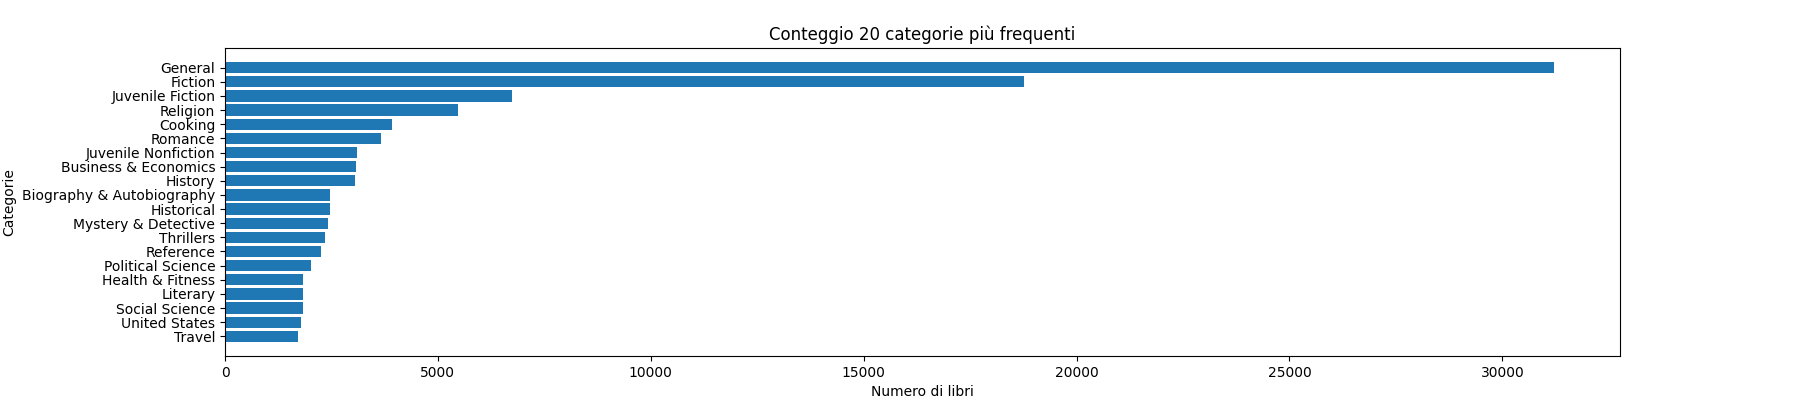
\includegraphics[width=1\textwidth]{pics/dati_iniziali.png}
    \caption{Database non bilanciato}
    \end{figure}
    
    \begin{justify}
    Dunque, per ovviare a problemi di overfitting, si è ritenuto necessario bilanciarlo quanto più possibile. Si passa dunque al seguente dataset:
    \end{justify}
    
    \begin{figure}[H]
    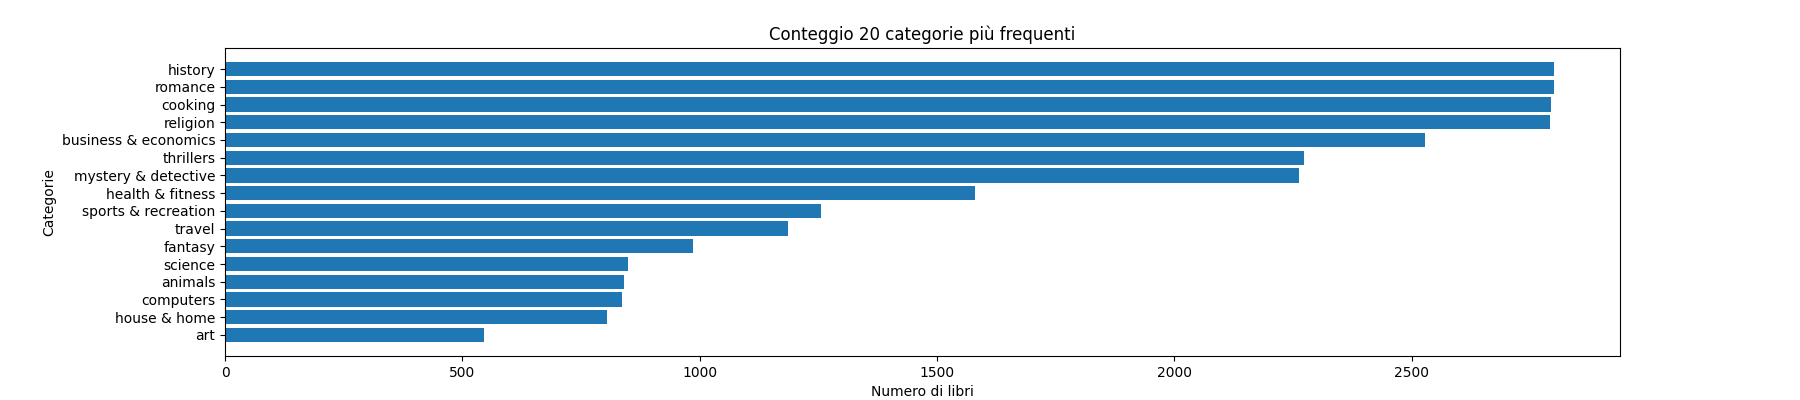
\includegraphics[width=1\textwidth]{pics/dati_postprocessati.png}
    \caption{Database bilanciato}
    \end{figure}
    
    \begin{justify}
    Come è possibile notare dalla 'Figure 2' il dataset non risulta completamente bilanciato. Questo risultato è dovuto alla natura stessa del dataset. Per ottenere un dataset bilanciato si sarebbero dovute eliminare molte informazioni, non avendo così più a disposizione abbastanza dati per addestrare i nostri modelli.\\
    \end{justify}
    \hfill
    \begin{justify}
    Il bilanciamento del dataset è stato effettuato tramite la funzione "balanceCategories", la quale verifica il numero di righe per ogni categoria ed elimina casualmente delle righe di categorie con più di 'threshold' esempi.
    \end{justify}
    \includegraphics[width=0.95\textwidth]{pics/balanceCategories.png}
    

    \begin{minipage}[t]{0.40\textwidth}
    \vspace{30pt}
    Possiamo concludere che sono state effettuate le seguenti modifiche del dataset in questione, con la rimozione del seguente numero di righe:
    \end{minipage}
    \hfill
    \begin{minipage}[t]{0.50\textwidth}
    \vspace{20pt}
    \includegraphics[width=1\textwidth]{pics/bilanciamento.png}
    \end{minipage}
    \end{enumerate}

    \hfill
    \hfill
    \begin{enumerate}
    \subsection{Visualizzazione Word Cloud}
    \begin{justify}
    Word Cloud è una tecnica per la visualizzazione dei dati. È utilizzata per rappresentare dati di testo in cui la dimensione di ciascuna parola ne indica l'importanza.\\
    Grazie all'utilizzo delle WordCloud, nello specifico tramite l'utilizzo delle funzioni "createDescriptionWordCloud" e "createAuthorsWordCloud", è stato possibile illustrare le parole chiavi presenti all'interno delle descrizioni e degli autori. Verrano creati tanti WordCloud quante sono le categorie.
    \end{justify}
    \includegraphics[width=0.95\textwidth]{pics/descriptionWordCloud.png}
    
    \newpage
    \begin{justify}
    La seguente immagine è un esempio di output della funzione (con lo scopo di farne comprendere il corretto funzionamento, vengono mostrate solo quattro categorie):
    \end{justify}
    \begin{figure}[H]
    \centering
    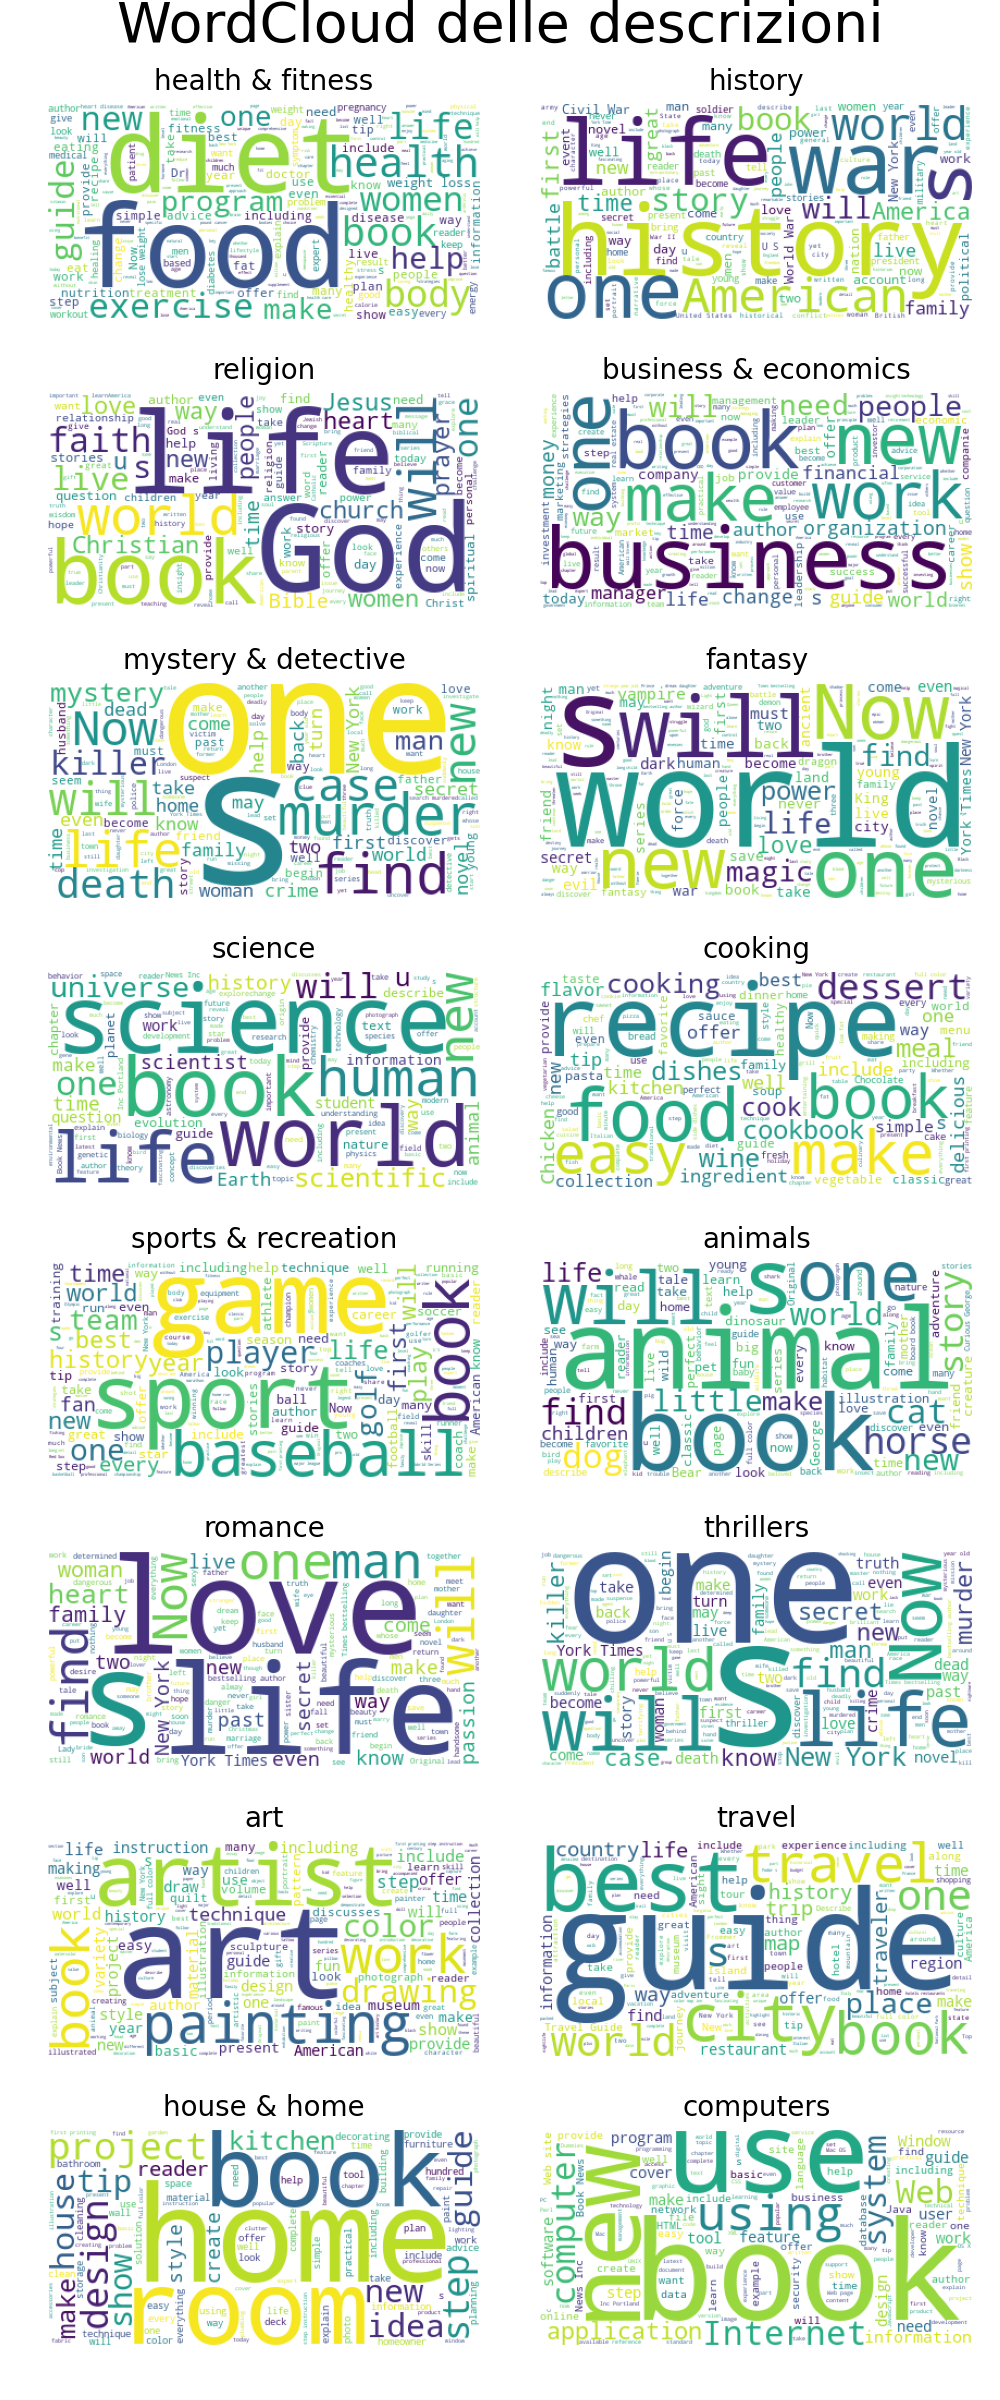
\includegraphics[width=0.90\textwidth]{pics/wordcloud_descrizioni_nonprocessate.png}
    \caption{Word Cloud delle descrizioni non processate}
    \end{figure}

    %\hfill
    \begin{justify}
    Tale illustrazione ci permette di analizzare con più semplicità le parole ricorrenti ed individuare delle stop words aggiuntive, che fanno riferimento al dataset in questione, come ad esempio "book" e "life". Allo stesso ragionamento vengono sottoposti gli autori.Per le stop words aggiuntive inerenti alla descrizione e agli autori sono stati creati due nuovi file di testo, chiamati rispettivamente "description\textunderscore{}stopwords.txt" e "authors\textunderscore{}stopwords.txt". Ecco le stop word individuate:
    \end{justify}
    %\includegraphics[width=0.10\textwidth]{pics/aggiuntaStopWordsDescription.png}
    
    \begin{figure}[H]
    \begin{subfigure}{0.15\textwidth}
    \includegraphics[width=\linewidth]{pics/aggiuntaStopWordsDescription.png} 
    \begin{justify}
    \caption{Stop Word delle descrizioni}  
    \end{justify}
    \label{fig:subim1}
    \end{subfigure}
    \hspace{3cm}
    \begin{subfigure}{0.17\textwidth}
    \includegraphics[width=\linewidth]{pics/aggiuntaStopWordsAutori.png}
    \begin{justify}
    \caption{Stop Word degli autori}   
    \end{justify}
    \label{fig:subim2}
    \end{subfigure}
    \caption{Stop Word aggiunte}
    \end{figure}

    \newpage
    \begin{justify}
    Con la successiva eliminazione delle stop words individuate, si ottiene il seguente word cloud:
    \end{justify}
    \begin{figure}[H]
    \centering
    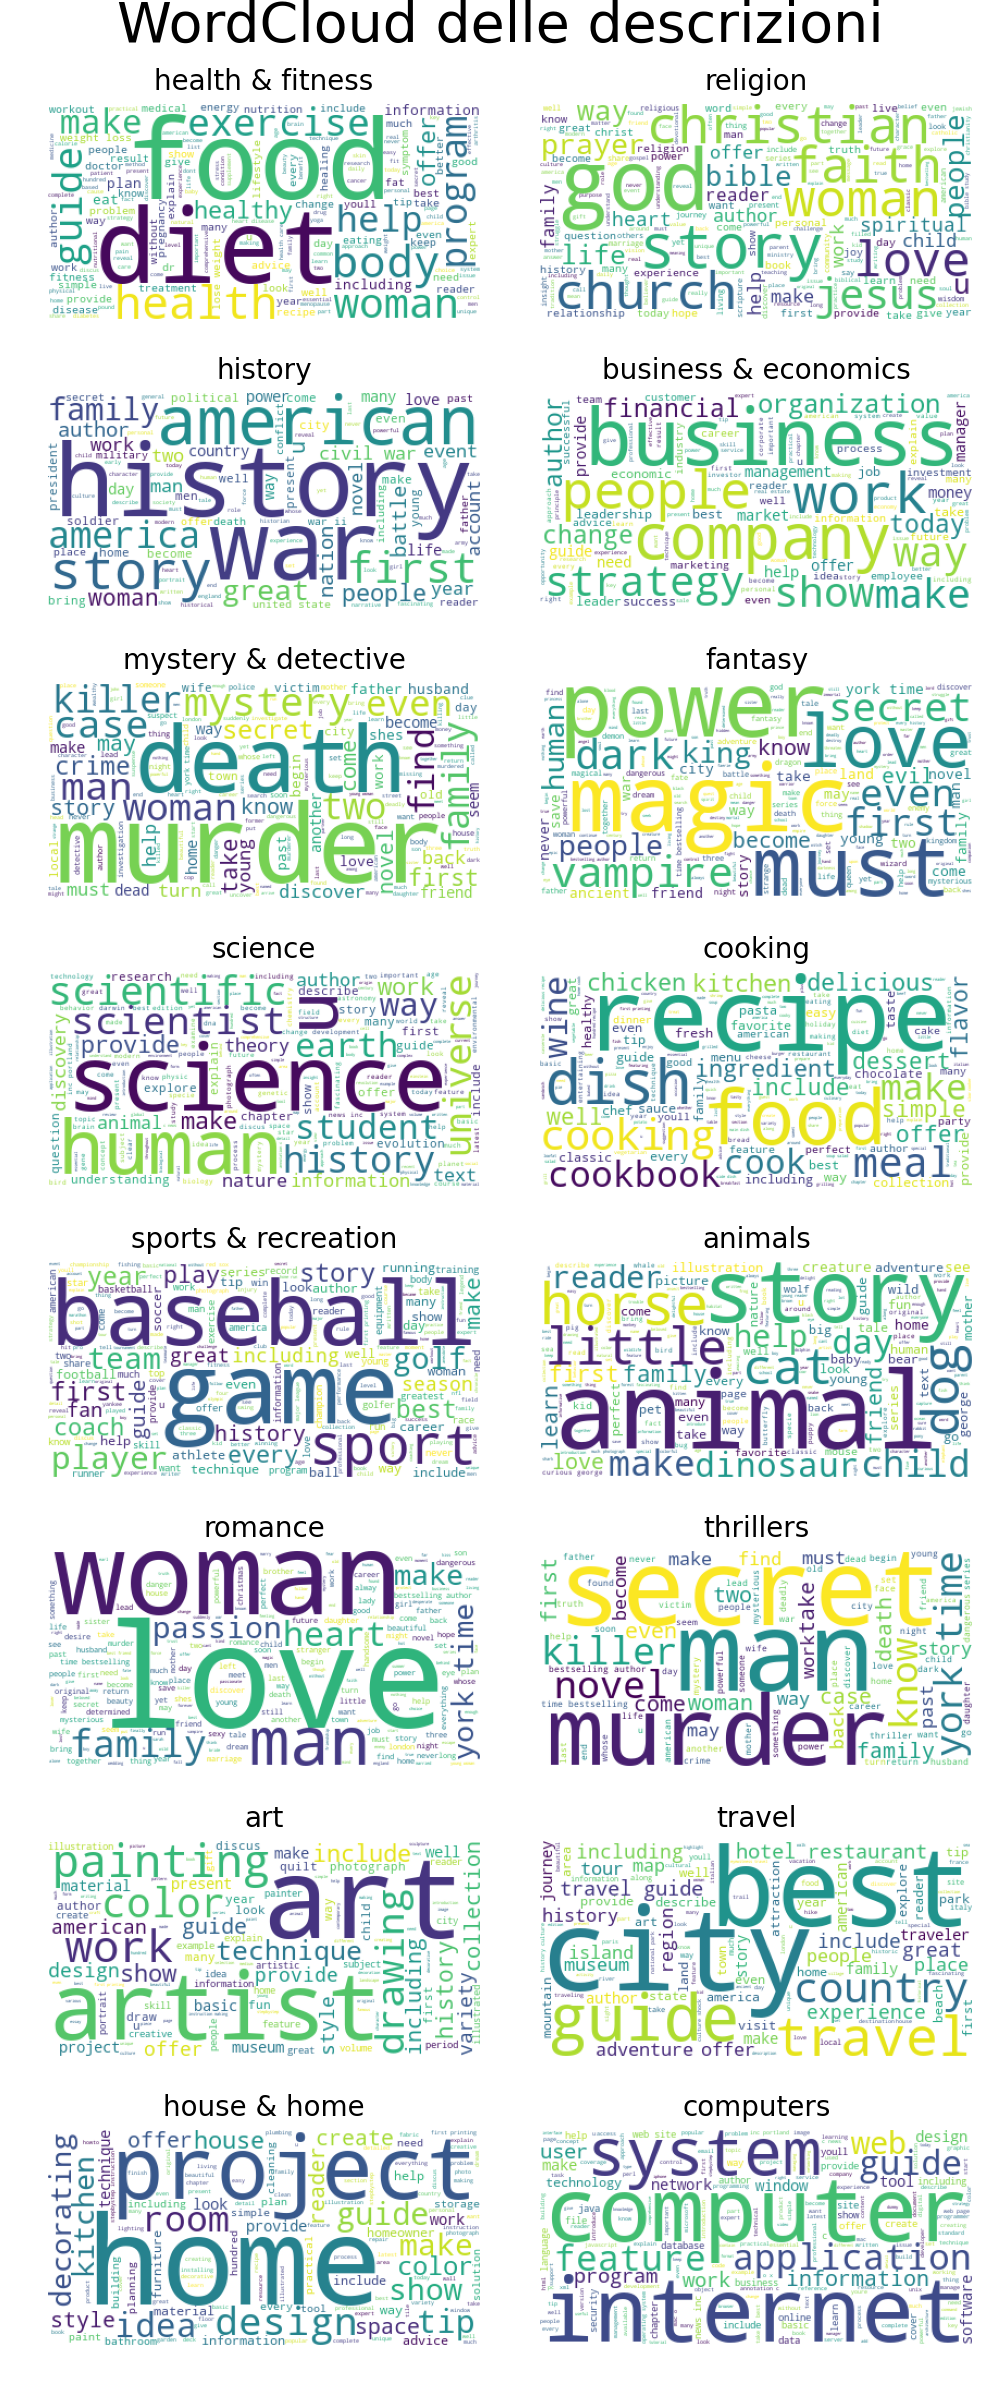
\includegraphics[width=0.95\textwidth]{pics/wordcloud_descrizioni_processate.png}
    \caption{Word Cloud delle descrizioni processate}
    \end{figure}

    \hfill
    \hfill
    \begin{figure}[H]
    \begin{subfigure}{0.48\textwidth}
    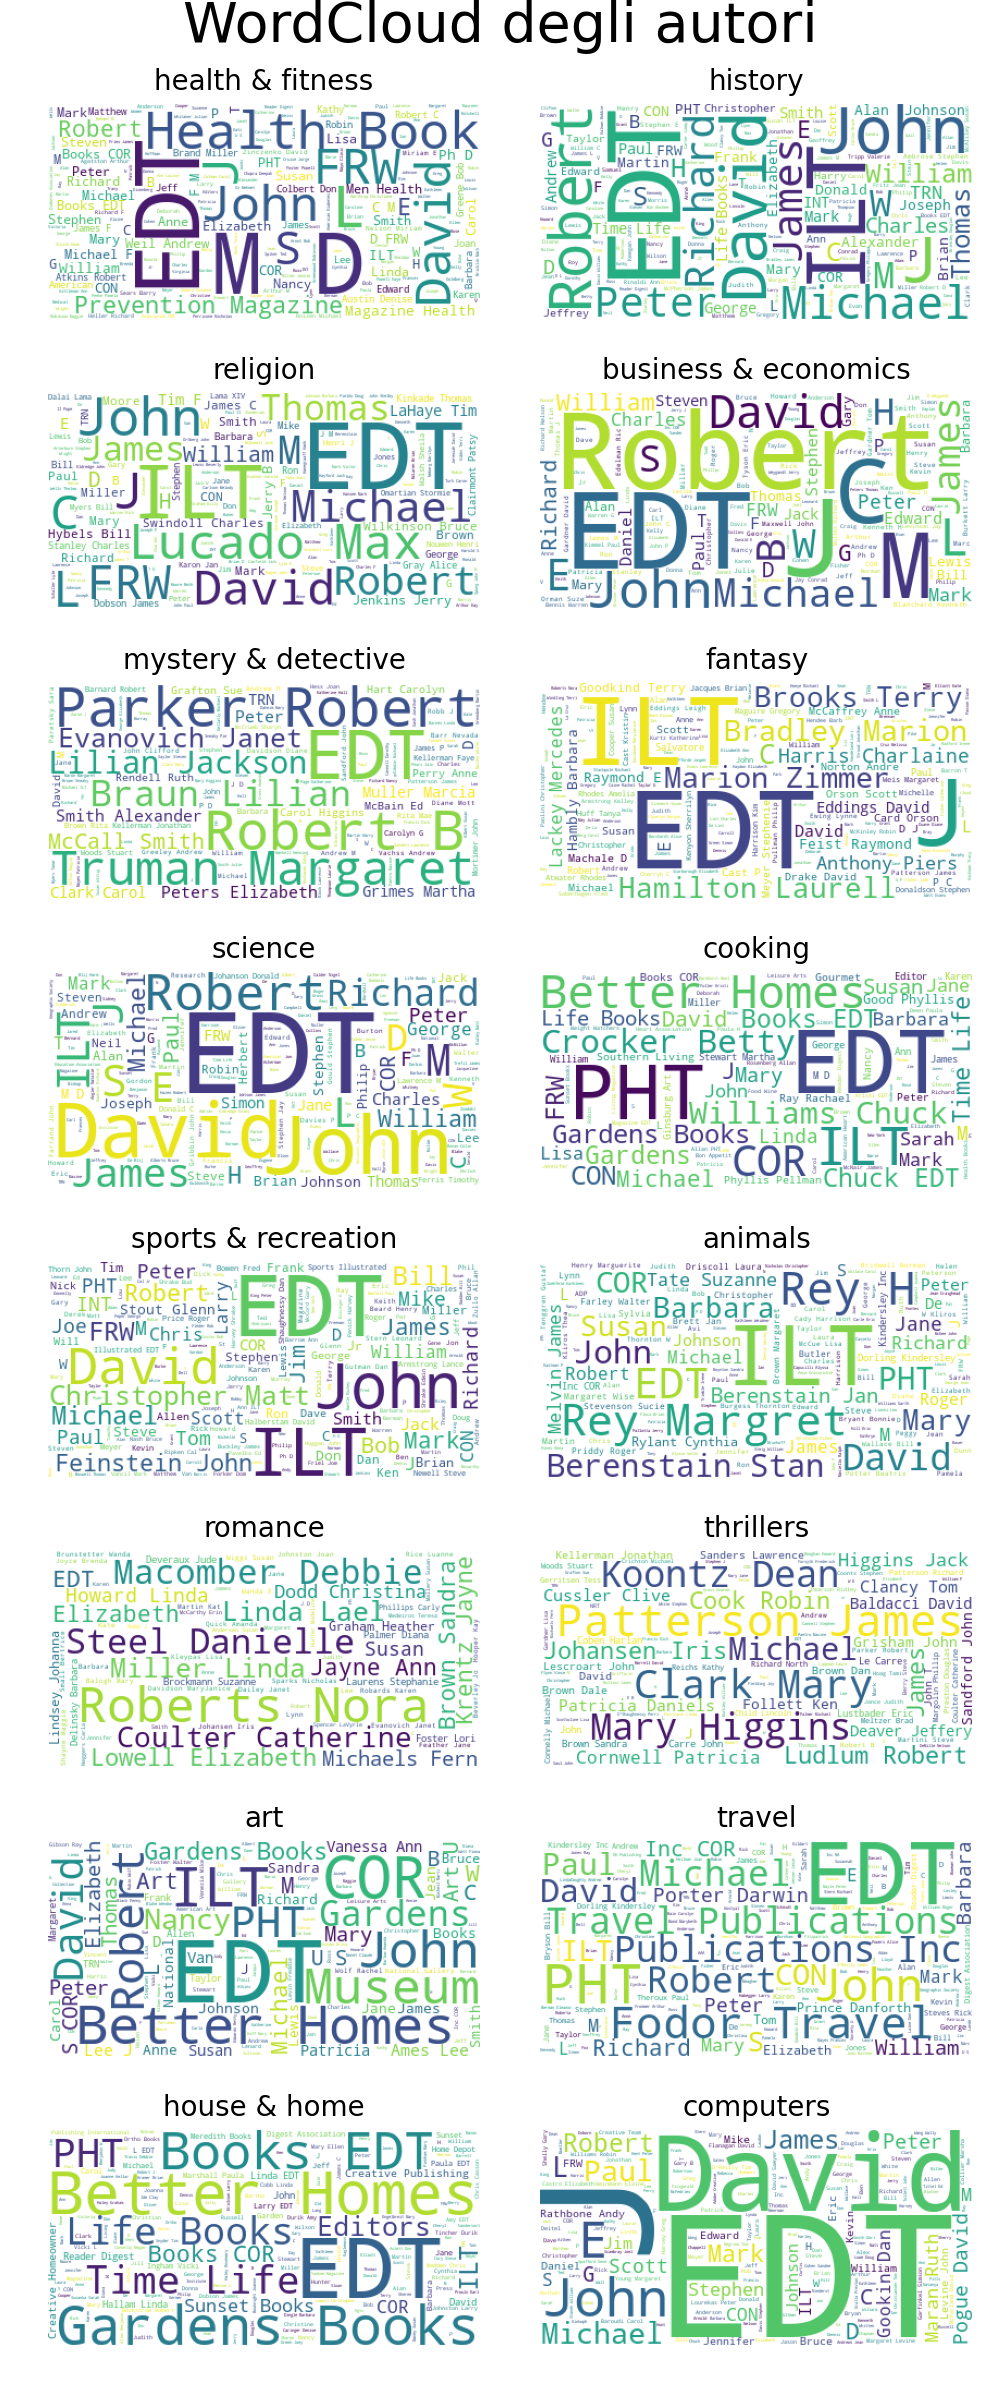
\includegraphics[width=\linewidth]{pics/wordcloud_autori_nonprocessati.png} 
    \caption{Word Cloud degli autori non processati}
    \label{fig:subim1}
    \end{subfigure}
    \begin{subfigure}{0.48\textwidth}
    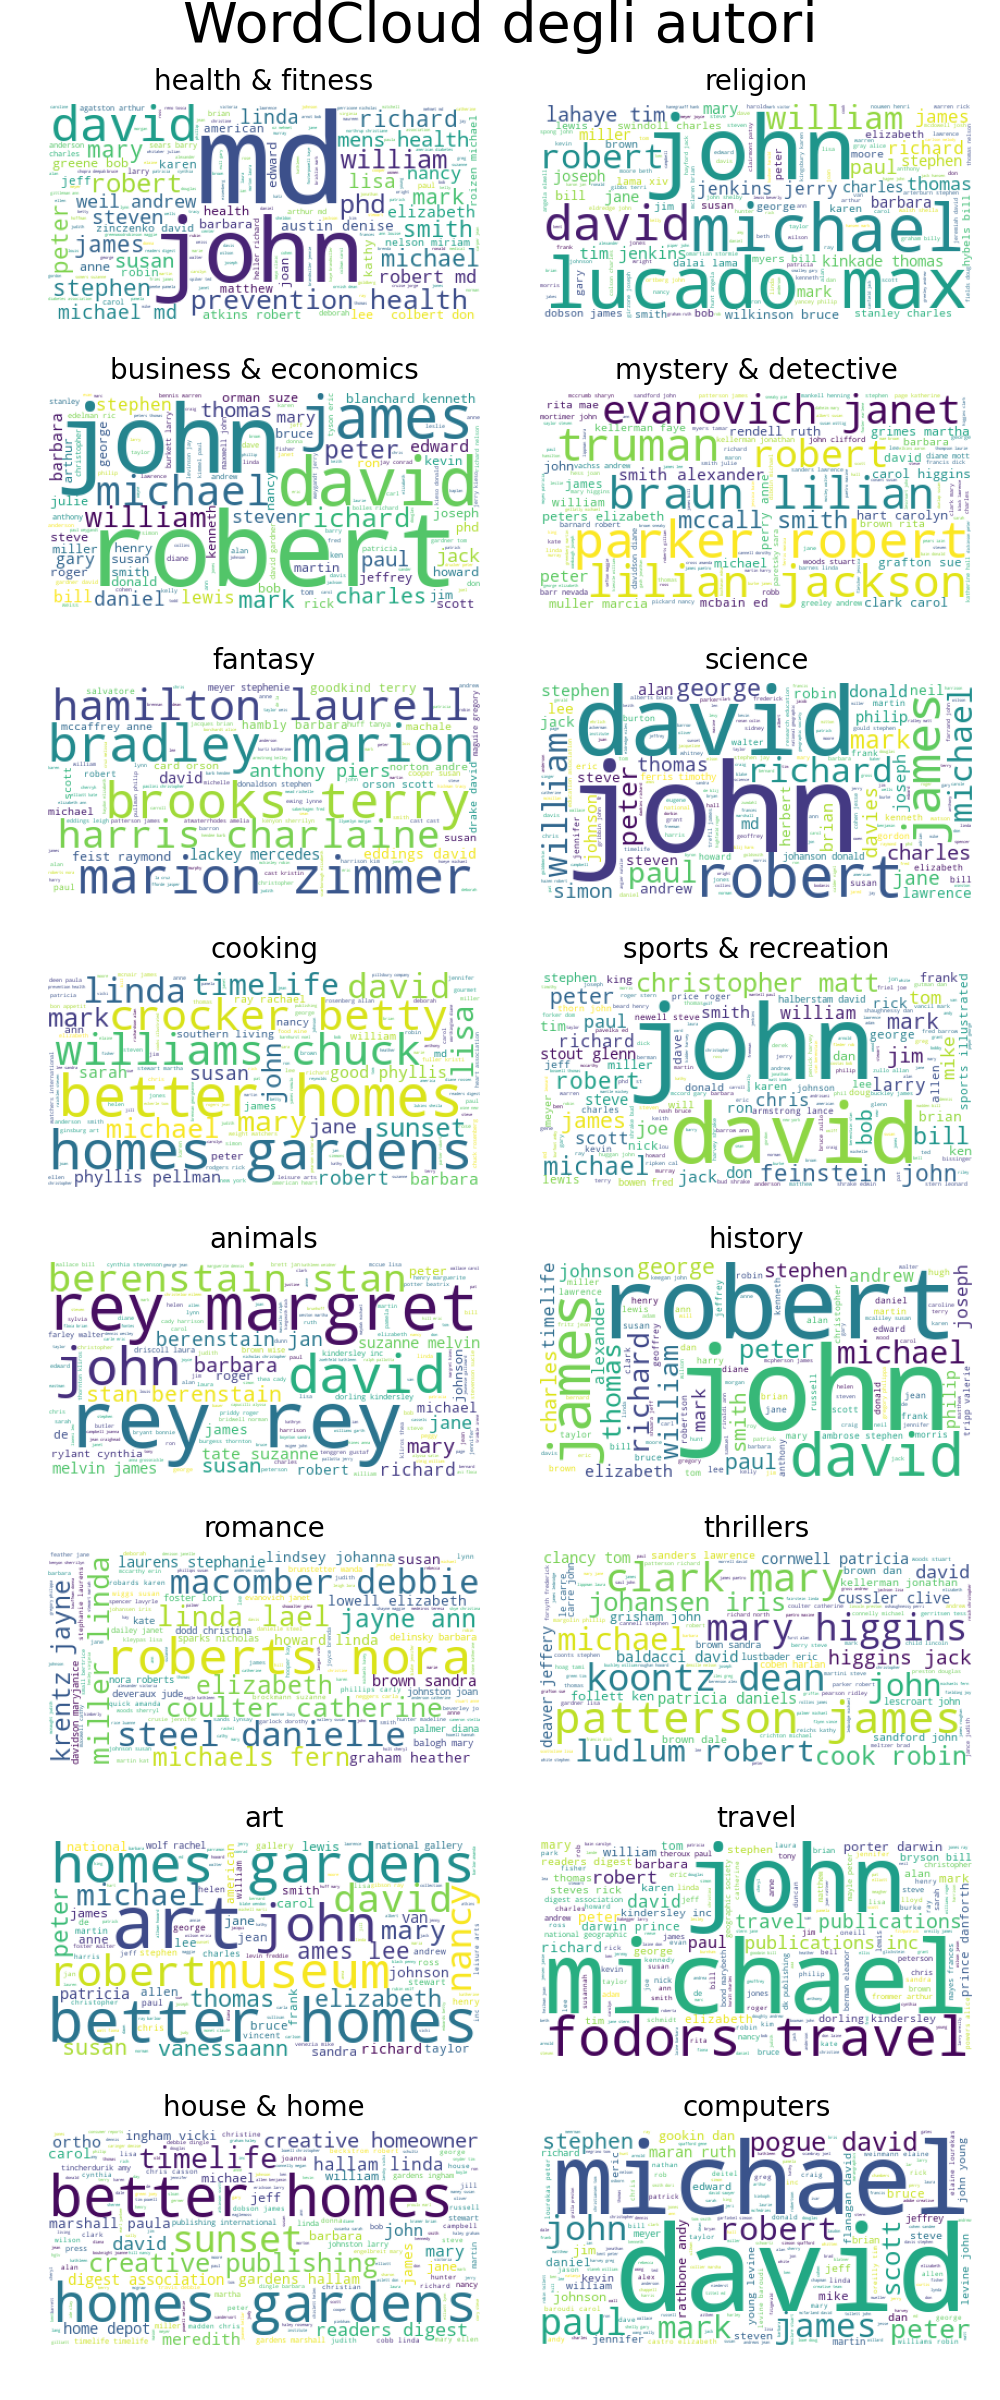
\includegraphics[width=\linewidth]{pics/wordcloud_autori_processati.png}
    \caption{Word Cloud degli autori processati}
    \label{fig:subim2}
    \end{subfigure}
    \caption{Word Cloud degli autori}
    \end{figure}
    \end{enumerate}



    \begin{enumerate}
    \subsection{Formattazione dei dati}
    \begin{justify}
    Il dataset utilizzato è composto da soli dati testuali ma per appiclare tecniche di machine learning è necessario formattarli. Abbiamo scelto di utilizzare TF-IDF come tecnica per elaborare il linguaggio naturale utilizzato per rappresentare i dati. TF-IDF sta per Term Frequency-Inverse Document Frequency infatti si occupa di calcolare due valori: la frequenza di una parola nel documento e quanto una parola è unica in tutti i documenti. Nel codice viene implementato il TfidfVectorizer che avrà come output una matrice, composta da valori di tf-idf, la quale è una rappresentazione numerica dei dati che serviranno per lo studio dello scopo del progetto. 
    \end{justify}
    \end{enumerate}


\section{Classificazione}

    \begin{enumerate}
    \subsection{Linear Support Vector Classification  }
    \end{enumerate}
   
    \begin{enumerate}
    \subsection{Mulinomial Classification}
    \end{enumerate}
    
     \begin{enumerate}
    \subsection{Complement Naive Bayes Classification}
    \end{enumerate}
    
    \begin{enumerate}
    \subsection{Logistic Classification}
    \end{enumerate}

    \begin{enumerate}
    \subsection{Stochastic Gradient Descent Classification}
    \end{enumerate}

   
    
    \begin{enumerate}
    \subsection{Valutazione della Classificazione}
    \end{enumerate}


\section{Clustering}
    \begin{justify}
        Allo scopo di effettuare un confronto più coerente con gli algoritmi di Classificazione, sono stati selezionati degli algoritmi di Clustering per cui il numero di cluster venisse impostato a priori. I modelli selezionati e addestrati sul dataset sono stati: K-Means, Mini-Batch KMeans e Spectral Clustering.
    \end{justify}
    \begin{enumerate}
    \subsection{Algoritmo K-Means}
    \begin{justify}
        L'algoritmo K-Means ha la funzione di assegnare oggetti ad un determinato cluster in modo che ci sia omogeneità tra gli oggetti nello stesso cluster ed eterogeneità tra gli oggetti in cluster diversi. È possibile descrivere questo algoritmo tramite i seguenti step:\\
    1) Scegliere in modo casuale K punti nel dataset che saranno i centroidi iniziali;\\
    2) Generare un partizionamento assegnando ogni campione al centroide più vicino;\\
    3) Calcolare i nuovi centroidi del cluster considerando la media dei valori del cluster generato al punto 2;\\
    4) Ripetere i passi 2 e 3 fino a quando i centroidi non varieranno più.
    \end{justify}
    \end{enumerate}

    \begin{enumerate}
    \subsection{Algoritmo MiniBatchKMeans}
    \begin{justify}
         L'algoritmo MiniBatchKMeans è una variante dell'algoritmo K-Means standard che utilizza minibatch, ovvero sottoinsiemi di dati di input campionati casualmente in ogni iterazione di training, di campioni per aggiornare i centroidi invece di utilizzare l'intero set di dati. Questo approccio rende Mini-Batch K-Means più efficiente computazionalmente, permettendo di lavorare su dataset più grandi. A differenza di altri algoritmi che riducono il tempo di convergenza, il mini-batch kmeans produce risultati che generalmente risultano leggermente peggiori rispetto all’algoritmo standard. È possibile descrivere l'algoritmo in questione tramite i seguenti step:\\
    1) Scegliere in modo casuale K punti nel dataset che saranno i centroidi iniziali;\\
    2) Selezionare casualmente un minibatch di dimensione prefissata dal dataset, generare un partizionamento           assegnando ogni suo campione al centroide più vicino e infine aggiornare i centroidi usando la media dei punti nel minibatch corrente;\\
    3) Per ciascun cluster, calcolare i nuovi centroidi come la media dei punti assegnati a quel cluster;\\
    4) Ripetere i passi 2 e 3 fino a quando i centroidi non varieranno più.
    \end{justify}
    \end{enumerate}

    \begin{enumerate}
    \subsection{Algoritmo SpectralClustering}
    \begin{justify}
        L'algoritmo SpectralClustering sfrutta il concetto di teoria spettrale (legata allo studio delle funzioni analitiche) e consente la gestione di strutture complesse e non lineari di dati. Utilizza la similarità tra i punti del dataset per costruire un grafo, per poi trasformarlo in uno spazio di dimensioni inferiori attraverso una procedura basata sugli autovettori. Infine, applica un algoritmo di clustering (ad esempio K-Means) nello spazio trasformato per raggruppare i punti in cluster.
    \end{justify}
    \end{enumerate}

    \begin{enumerate}
    \subsection{Valutazione del Clustering: Silhouette score}
    \begin{justify}
        Allo scopo di valutare gli algoritmi di clustering ne è stato calcolato il rispettivo Silhoutte score, il cui valore oscilla tra -1, per clustering errato, e +1, per clustering altamente denso. Invece i punteggi intorno allo 0 indicano la presenza di clusters sovrapposti. 
        In seguito, si ha avuto cura di ricercare in maniera randomica gli iperparametri migliori del modello con lo score più alto.
    \end{justify}
    \end{enumerate}

\section{Conclusioni}

    
\end{document}
